\subsection{Fisher Information}
\label{subsec:fim}
Under~\eqref{eq:observation}, the Fisher information matrix (FIM) of the position is:
\begin{equation}
 \vect I(\vect r)=\vect J\trans\vect W\vect J,\qquad
 \vect W=\diag\!\left(\frac{L}{\sigma_1^2},\ldots,\frac{L}{\sigma_K^2}\right),
 \label{eq:fim}
\end{equation}
where the rows of $\vect J\in\R^{K\times3}$ are the gradients $\nabla s_i\trans$, and the position error bound (PEB) is $\mathrm{PEB}=\sqrt{\operatorname{tr}\vect I^{-1}}$. With the common noise level $\sigma$ used in the experiments, $\vect W=(L/\sigma^2)\,\vect I_K$. With $\vect P_{\vect u}=\vect I_3-\vect u\vect u\trans$, $\nabla d=-\vect u$ and $\partial\vect u/\partial\vect r=-\vect P_{\vect u}/d$, the separable form~\eqref{eq:separable} gives:
\begin{equation}
 \nabla s_i=R(\psi_i)\nabla\beta-\frac{\beta}{d}\dot R(\psi_i)\left(\vect n_i-\cos\psi_i\,\vect u\right),
 \label{eq:gradient}
\end{equation}
where $\dot R(\psi)=\mathrm dR/\mathrm d(\cos\psi)$ is the derivative of the response with respect to the incidence cosine and, for the Lambertian pattern:
\begin{equation}
 \nabla\beta=\frac{\beta}{d}\left[(m+2)\,\vect u-\frac{m}{\cos\phi}\,(-\vect n_t)\right].
 \label{eq:beta-gradient}
\end{equation}
The first term of~\eqref{eq:gradient} is common to all orientations and carries range information; the second depends on the orientation and carries direction information. For the SQ response, $\dot R(\psi)=2a\psi/\sin\psi$ inside its support, with $\dot R(0)=2a$; the information is therefore set by the \emph{slope} of the response, not by its value. A response model that reproduces the measured amplitudes but not their slope can produce misleading bounds and estimates.

\subsection{Local Identifiability}
\label{subsec:identifiability}
Let $\vect E\in\R^{3\times2}$ be an orthonormal basis of the plane orthogonal to $\vect u$. In the illuminated region, the map from $\vect r$ to the local coordinates $(\ln\beta,\bm\omega)$, where $\bm\omega$ are two tangent coordinates of $\vect u$, is invertible, and therefore:
\begin{equation}
 \operatorname{rank}\vect J=\operatorname{rank}\left[\,\vect R,\ \diag(\dot{\vect R})\,\vect N\trans\vect E\,\right],
 \label{eq:rank}
\end{equation}
with $\vect R=[R(\psi_1),\ldots,R(\psi_K)]\trans$, $\dot{\vect R}$ defined likewise and $\vect N=[\vect n_1,\ldots,\vect n_K]$. The position is locally identifiable if this $K\times3$ matrix has rank three. Three consequences guide the experiment.

First, at least three illuminated orientations are needed, but they are not sufficient: the tangent projections $\vect E\trans\vect n_i$, weighted by the response slope, must span the plane orthogonal to $\vect u$. If the PD normal coincides with the rotation axis of the stage, all incidence angles are equal and~\eqref{eq:rank} has rank one; turning an untilted PD provides no information. The receiver must be \emph{tilted} with respect to the rotation axis. For the cosine family, homogeneity reduces~\eqref{eq:rank} to the rank of the illuminated normals; for a nonhomogeneous response such as SQ this reduction does not hold, and~\eqref{eq:rank} must be checked directly. Local identifiability does not imply global uniqueness either: with coplanar normals, the SQ model can admit two symmetric solutions with a finite bound, which is why the estimator of Section~\ref{subsec:estimator} uses several starting points.

Second, the direction stage needs neither $A$ nor the LED pattern, which only scale the amplitude column. The distance, in contrast, is only available through $\beta$: if $A$ were unknown, $\beta$ and $d$ could not be separated, and reorientation alone cannot remove this distance--gain ambiguity. The calibration of $A$ and $m$ is therefore not a refinement but a condition for three-dimensional positioning.

Third, the information depends on the response slope at the incidence angles actually visited, which links the tilt of the receiver to the attainable accuracy.

\subsection{Role of the Receiver Tilt}
\label{subsec:tilt}
The axial case makes this link explicit. Consider a vertical LED, the PD on its axis at distance $d$, and $K\geq3$ normals uniformly spaced in azimuth on a cone of half-angle $\theta$ about the vertical, all illuminated, with a common noise level $\sigma$. The FIM is diagonal:
\begin{equation}
 \vect I=\frac{LKA^2}{\sigma^2d^6}\diag\!\left(\frac{\dot R^2\sin^2\theta}{2},\ \frac{\dot R^2\sin^2\theta}{2},\ 4R^2\right),
 \label{eq:axial-fim}
\end{equation}
with $R$ and $\dot R$ evaluated at $\psi=\theta$, and the bound is:
\begin{equation}
 \mathrm{PEB}^2=\frac{\sigma^2d^6}{LKA^2}\left[\frac{4}{\dot R(\theta)^2\sin^2\theta}+\frac{1}{4R(\theta)^2}\right].
 \label{eq:axial-peb}
\end{equation}
The horizontal terms decrease with $\sin\theta$ and with the response slope, and they diverge as $\theta\to0$; the vertical term is controlled by the response value, i.e., by the received amplitude. The bound grows as $d^3$, and repeating independent orientations improves it as $1/\sqrt{K}$ only when the records per orientation are fixed.

\subsection{Orientation Uncertainty}
\label{subsec:orientation-uncertainty}
The normals are never known exactly. Suppose that each normal is perturbed by an independent angular error with standard deviation $\sigma_\theta$ per tangent component, measured by an auxiliary sensor (the stage encoder or an IMU) and persisting over all the records of that orientation. Eliminating the orientation errors from the joint likelihood gives the effective FIM:
\begin{equation}
 \vect I_e=\vect J\trans\left(\bm\Sigma_y+\vect D\bm\Sigma_\theta\vect D\trans\right)^{-1}\vect J,\qquad
 \vect D_i=\beta\dot R(\psi_i)\,\vect u\trans\vect E_i,
 \label{eq:fim-orientation}
\end{equation}
where $\bm\Sigma_y=\vect W^{-1}$, $\vect E_i$ is a tangent basis at $\vect n_i$, and $\vect D_i$ is the $i$th block row of $\vect D$. For isotropic, independent errors this amounts to replacing the noise variance of each orientation by:
\begin{equation}
 \sigma_{i,\mathrm{eff}}^2=\frac{\sigma_i^2}{L}+\sigma_\theta^2\,\beta^2\dot R(\psi_i)^2\sin^2\psi_i.
 \label{eq:effective-variance}
\end{equation}
Orientation errors thus behave as signal-proportional noise that is not reduced by averaging records. At the high SNR of an amplified PD they dominate the bound, as shown next.

\subsection{Numerical Study of the Bound}
\label{subsec:design}
The bound is now evaluated in a generic indoor scenario, independent of the testbed of Section~\ref{sec:testbed}, to see how the tilt, the number of orientations and the main parameters of the link interact. An LED at a height of 3~m points down, with $P_t=0.65$~W and $\Phi_{1/2}=45^\circ$ ($m=2$). The PD has an area of 75.4~mm$^2$ and the SQ response~\eqref{eq:sq-response} with $\psi_{3\mathrm{dB}}=0.61$~rad, without aperture, and a common noise level gives an SNR of 475 to an untilted PD on the floor below the LED. The positions cover $X,Y\in[-1,1]$~m with 0.1~m spacing at seven heights from 0 to 1.8~m (3\,087 positions), from which the LED is seen at up to $\alpha_{\max}=49.7^\circ$ from the vertical. The $K$ normals are uniformly spaced in azimuth on a cone of tilt $\theta$, and the orientation errors follow Section~\ref{subsec:orientation-uncertainty}. The coverage is the fraction of positions with $\mathrm{PEB}\le10$~cm. Fig.~\ref{fig:sim} summarizes the results.

With exactly known normals, the tilt is not critical: for $K=5$, every position is covered from $\theta=3.5^\circ$, and the median bound at $15^\circ$ is 0.71~cm (Fig.~\ref{fig:sim}(a)). Orientation errors change this picture. Their contribution to~\eqref{eq:effective-variance} grows with the signal, so they set a floor that neither power nor averaging can lower, and the tilt becomes the main design variable. With $\sigma_\theta=1^\circ$, the median bound at $15^\circ$ rises to 5.5~cm, and covering every position with $K=5$ requires $\theta\ge14^\circ$ (Fig.~\ref{fig:sim}(b)). More orientations relax this requirement, down to $9.5^\circ$ for $K=10$, whereas three orientations never cover more than 98.8\,\% of the positions. The required tilt also follows the uncertainty: $7.5^\circ$ suffice for $K=5$ with $\sigma_\theta=0.5^\circ$, and with $\sigma_\theta=2^\circ$ no tilt covers the volume with $K\le10$.

The field of view limits the tilt from above. On a cone of tilt $\theta$, the largest incidence angle is close to $\alpha_{\max}+\theta$, so the LED stays inside the $64.6^\circ$ support of the SQ response for all orientations and positions only up to $\theta\approx15^\circ$; at $30^\circ$, one position in ten has an orientation that misses the LED (Fig.~\ref{fig:sim}(b)). The bound tolerates such losses, and with $K=5$ the coverage stays above 98\,\% up to $45^\circ$, but the estimator then depends on the response near its cutoff, where the signal is weakest and the model is not differentiable. An aperture narrower than the support lowers this limit by the same amount. Larger tilts gain little in exchange: with $\sigma_\theta=1^\circ$, the median bound reaches its minimum at about $30^\circ$, only 25\,\% below its value at $15^\circ$.

The beam of the LED matters mostly through the orientation errors (Fig.~\ref{fig:sim}(c)). A narrow beam makes the received amplitude depend strongly on the direction, so that direction errors leak into the distance, as quantified in~\eqref{eq:range-sensitivity}: at $\theta=15^\circ$ and with $\sigma_\theta=1^\circ$, every position is covered only for $\Phi_{1/2}\ge37.5^\circ$, against $22.5^\circ$ with exactly known normals. The PD area, the transmitted power and the noise level, finally, enter the bound only through the ratio $A/\sigma$ (Fig.~\ref{fig:sim}(d)). With exactly known normals the bound decreases as $\sigma/A$, as in~\eqref{eq:axial-peb}; with orientation errors it saturates, and beyond a few tens of square millimeters a larger detector, a brighter LED or a quieter receiver no longer improves it.

The tilt must therefore lie in a window, bounded from below by the orientation uncertainty and from above by the field of view. In this scenario both edges lie close to $15^\circ$: covering the volume with $K=5$ and $\sigma_\theta=1^\circ$ requires at least $14^\circ$, and keeping the LED inside the response of every orientation allows at most $64.6^\circ-49.7^\circ\approx15^\circ$. At $\theta=15^\circ$, the bound stays below 9.2~cm at every position, with medians from 6.1~cm on the floor to 5.1~cm at 1.8~m. This is the tilt of the receiver used in the experiments (Section~\ref{subsec:hardware}); the bound of the actual testbed, with its calibrated model and measured noise, is compared with the measured errors in Section~\ref{subsec:res-bound}.

\begin{figure*}[!t]
 \centering
 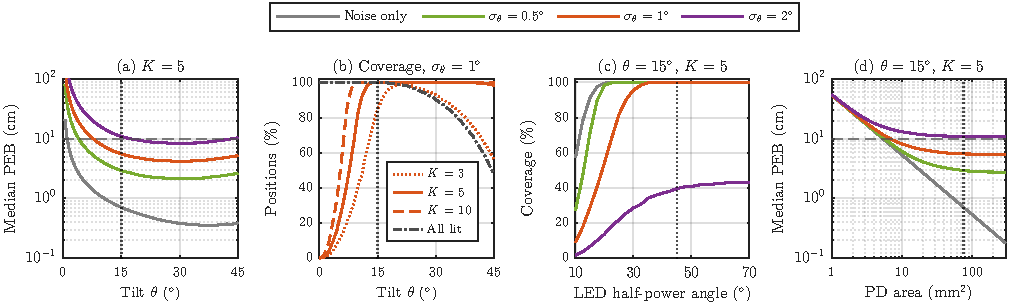
\includegraphics[width=\textwidth]{fig_sim.pdf}
 \caption{Position error bound in the generic scenario of Section~\ref{subsec:design}: LED 3~m above the floor, PD positions over $2\times2$~m at heights from 0 to 1.8~m, SQ response, and $K$ normals on a cone of tilt $\theta$. Colors give the orientation uncertainty $\sigma_\theta$. (a)~Median bound versus the tilt, $K=5$. (b)~Coverage ($\mathrm{PEB}\le10$~cm) versus the tilt for $\sigma_\theta=1^\circ$, and fraction of positions at which all five orientations see the LED (all lit). (c)~Coverage versus the half-power angle of the LED and (d)~median bound versus the PD area, at $\theta=15^\circ$ with $K=5$. Dotted lines: values of the scenario; dashed lines: 10~cm.}
 \label{fig:sim}
\end{figure*}
